\documentclass[../main.tex]{subfiles}
\graphicspath{{\subfix{../images/}}}
\begin{document}
\section*{Term 1 Week 8}
\begin{enumerate}
    \item 
    A circle of radius 1 whose centre is on the y-axis is normal to the parabola \(y=x^2\) as shown in the figure.\\
    Find the y-coordinate of the centre of the circle.\\
    \begin{figure}[h]
        \centering
        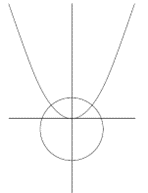
\includegraphics{images/t1w8q1.png}

    \end{figure}

    \item 
    Find an exact expression involving surds for \(\sin{(18\text{\textdegree})}\)\\

    \item 
    A circle of radius 1 is drawn tangent to the x-axis and to the line \(y=x\).\\
    
    A sequence of circles is then added with each new circle being tangent to the previous one and to the two lines as indicated in the diagram.\\
    
    Find the ratio of the areas of two adjacent circles in this sequence.\\
    \begin{figure}[h]
        \centering
        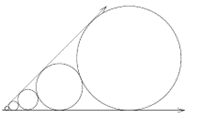
\includegraphics{images/t1w8q3.png}
    \end{figure}

    
\end{enumerate}

\end{document}